\section{Methods}  \label{sec:Methods}

%%%%%%%%%%%%%%%%%%%%%%%%%%%%%%%%%%%%%%%%%%%%%%%%%
\subsection{Physical Model for X-Ray Near-field Holotomography} \label{subsec:physics}
In holographic measurements, as e.g. conducted at synchroton facilities there are different conventions in how to define the forward model.
Assuming objects with a slowly varying phase or single material, it is possible to linearize the model \cite{zablerOptimizationPhaseContrast2005}.
To have a framework which keeps the non-linearity of the forward model and hence allows to reconstruct large phase-shifts without the need for unwrapping we follow Wittwer \textit{et al.} \cite{wittwerPhaseRetrievalFramework2022}.\\
The sample is characterized via the \textit{refractive index}
\begin{equation}
  n(x,y,z) = 1 - \delta(x,y,z) + \im \beta(x,y,z),
  \label{eq:refr_idx}
\end{equation}
where $\delta$ and $\beta$ describe the phase-shifting and absorption property of the material at a point $(x,y,z) \in \mathbb{R}^3$.
To simplify the notation we define the \textit{refractive object} by
\begin{equation}
  O(x,y,z) := \delta(x,y,z)  - \im \beta(x,y,z).  
\label{eq:refr_obj}
\end{equation}
We then assume that the model is sufficiently thin to model the interaction with the X-rays via a projection along the rays, which is commonly referred to as \textit{projection
approximation} \cite[ch.~2.2]{paganinCoherentXrayOptics2006}.
The wave field after the interaction of the incoming wave field \(  \Psi_{0} \) with the object \( O \) is given by
\begin{equation}
  \Psi_\varphi (O, \Psi_{0})(x,y) = \exp \left( -\im k \int_{\ell_{\varphi,x,y}}
  O(\textbf{x})
\mathrm{d}\mathbf{x} \right)   \, \Psi_0(x,y),
\label{eq:exit_wave}
\end{equation}
where we have the angular wave number \( k=\frac{2\pi}{\lambda} \) for wave length \(  \lambda. \)
Here, the line along which we integrate
\begin{equation}
  \ell_{\varphi,x,y} = \left\{  (\tilde{x},\tilde{y},\tilde{z}) \in \mathbb{R}^3: \tilde{y}=y,
    \,  \tilde{x} \cos\varphi + \tilde{z} \sin\varphi = x \right\}
\label{eq:ray_line}
\end{equation}
is the set of points of the ray hitting the detector at $(x,y)$ when the sample is rotated by $\varphi$.
\\
The illumination is modeled similar to the object, i.e. for the incoming wave
field $\Psi_0$ we have
\begin{equation}
  \Psi_0 (x,y) = \exp \left(-  \im \psi_0(x,y) + a_0(x,y) \right)  .
\label{eq:incoming_wave_field}
\end{equation}
As all angles in a holotomography scan are acquired consecutively we assume a
constant probe for the whole dataset, independent of the angle $\varphi \in
[0, \pi)$. \\
The propagation of the exiting wave field $\Psi_\varphi$ is then described by
the \textit{Fresnel Propagator} \( \mathcal{D}_\mathrm{Fr} \) and the measurement \( \mathcal{I}_{\mathrm{det}, \varphi}
\) is the squared magnitude of the propagated wave field, i.e. the phase
information gets lost
\begin{align}
  \mathcal{D}_\mathrm{Fr} \left( \Psi_\varphi \right) &=  \mathcal{F}^{-1} \left( \exp \left( -\mathrm{i} \pi \frac{k_x ^2 +
  k_y ^2}{\mathrm{Fr}} \right) \mathcal{F}\left( \Psi_\varphi \right)   \right)  \\
        \mathcal{I}_{\mathrm{det}, \varphi} &= \left| \mathcal{D}_\mathrm{Fr}\left( \Psi_\varphi \right)  \right| 
  ^2.
  \label{eq:propagation}
\end{align}
In \eqref{eq:propagation} we have the \textit{Fourier transform} \(  \mathcal{F} \) and it inverse \(  \mathcal{F}^{-1} \), \( k_x \) and \( k_y \) are the coordinates in the frequency domain.
The \textit{Fresnel number} \( \mathrm{Fr} \) which is given by

\begin{equation}
  \mathrm{Fr} = \frac{a^2}{\lambda M z_{12}}
\label{eq:Fresnel_nr}
\end{equation}
accounts for the geometry and other physical properties.
We have the characteristic feature size $a$, typically the voxel size in the object and the magnification $M = \frac{z_{02}}{z_{01}}$ which gives access to the
nanometer regime, despite the pixels on the detector being significantly larger.
The distances \( z_{ij} \) are described in \cref{fig:beam}.
\begin{figure}[htbp]
 \centering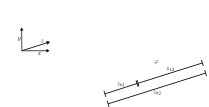
\includegraphics[width=11cm]{imgs/Beam.pdf}
 \caption{The setup of holotomography with the distances \( z_{01} \) between focal point and sample, \( z_{12}  \) between sample and detector and \( z_{02} \) between focal point and detector.}
 \label{fig:beam}
\end{figure} \\
Similarly to the holograms \( \mathcal{I}_{\mathrm{det}, \varphi} \) of the object, we obtain \textit{flat-field} or \textit{empty measurements} \( \mathcal{I}_{\mathrm{det}, \emptyset} \) by propagating the incoming wave field to the detector, i.e.
\[
  \mathcal{I}_{\mathrm{det}, \emptyset} = \left| \mathcal{D}_\mathrm{Fr} \left( \Psi_0 \right)   \right|^2. 
\] 
To simplify the problem it is common to account for the probe via a \textit{flat-field correction} \cite{doraArtifactsuppressingReconstructionStrongly2024} that assumes 
\[
  \left|  \mathcal{D}_\mathrm{Fr} \left( \exp \left( -\mathrm{i} k \int_{\ell_{\varphi,x,y}} O(\textbf{x}) \mathrm{d}\textbf{x} \right)  \right) \right|^2 \approx \frac{\mathcal{I}_\mathrm{det, \varphi}}{\mathcal{I}_\mathrm{det, \emptyset}},
\]
which is valid for (nearly) constant empty measurements \( \mathcal{I}_\mathrm{det, \emptyset} \), but introduces errors for a rapidly varying probe which results in reconstructions that suffer from artifacts \cite{nikitinXrayNanoholotomographyReconstruction2024}.
In \cref{sec:results_syn} we will also see an example motivating the accurate modeling of the physics as in \eqref{eq:propagation}.
After describing the acquisition process and emphasizing the need of accurate modeling we want to recall that our goal is to
recover the refractive object \(O\) and the incoming wave field \(
\Psi_{0} \) from the measurements \( \mathcal{I}_{\mathrm{det}, \varphi} \) and \( \mathcal{I}_{\mathrm{det}, \emptyset} \), i.e.
solving the coupled inverse problem of phase retrieval and tomography.



\subsection{Implicit Neural Representations with Multiresolution Hash Encoding} \label{subsec:INRs}
The idea behind INRs is to overcome the big memory requirement by pixel or voxel representations when aiming for a high resolution as well as being independent from grids.
As already mentioned in the Introduction~\ref{sec:Intro}, an appropriate architecture is fundamental to obtain good representations.
We will apply the configuration proposed by Müller \textit{et al.} \cite{mullerInstantNeuralGraphics2022} that was already introduced to the related inverse problems of cone beam CT \cite{ zhaNAFNeuralAttenuation2022} and holotomography without probe retrieval \cite{gruenXRayNearFieldHolotomography2026}.\\
The object is encoded \textit{spatially} using grids with levels \( 0, \dots, L-1 \) (coarse to fine) for multiple resolutions, as depicted in \cref{fig:hash_encoding} for two grids, and in 2D for simplicity.
\begin{figure}[htbp]
 \centering\includegraphics[width=\textwidth]{imgs/hash_encoding.pdf}
 \caption[Illustration of the used architecture.]{
   Illustration of a forward pass through the architecture.
   First, we obtain the 4 surrounding vertices which are hash encoded by \eqref{eq:hash_encoding} for the different levels.
   The corresponding entries in the lookup-table are then weighted by the proximity to \( x \) and summed up to obtain the input for the MLP, which yields the predicted values of the refractive object \eqref{eq:refr_obj} at position \( x. \) 
}
 \label{fig:hash_encoding}
\end{figure}
The extension to 3D is straightforward, i.e.
we have 8 surrounding nodes and then interpolate trilinear before feeding the encoded \( x \) to the MLP.
A forward pass through the architecture is started by relating the coordinate \( x \in \left[ 0, 1 \right]  \) to its surrounding nodes which are 
\[
\{ \hat{x}  \in  \mathbb{N}^3: \hat{x} _i \in \{ \left\lfloor x_i \cdot N_l \right\rfloor, \left\lceil x_i \cdot N_l \right\rceil \} \}  
\] 
For coarser grids with fewer nodes there is no need to limit the lookup-table, but as soon as the number of nodes exceeds the table size, \(  T \) we use a hash encoding 
\begin{equation}
  \begin{aligned}
  h \colon \mathbb{N}^3 \to \{0, \ldots , T-1 \}   \colon  \\
  \hat{x}\mapsto  \left(  \bigoplus_{n=1}^{3} \hat{x} _i \pi_i  \right) \mod T 
  \label{eq:hash_encoding}
  \end{aligned}
\end{equation}
and lose injectivity in favor of computational efficiency.
With \( \bigoplus \) we denote the bit-wise XOR operation, by chosing \( \pi=\begin{pmatrix} 1, \ 654 435 761, \ 805 459 861 \end{pmatrix}\) we decorrelate the dimensions.
After mapping the nodes to \(  \{0, \ldots, T-1\}   \) we get the corresponding entries in the lookup-table for all surrounding nodes and interpolate trilinear to account for locality.
The concatenated input of all levels is then fed into the 4-layer MLP which processes everything to give the final prediction of \(  \delta  \) and \(  \beta  \).\\
When \( N_0 \ll T \ll N_{0}\cdot b^{L-1} \) we can use stochastic arguments that the unique mapping on the first levels and the different collisions on the higher levels make this representation robust and for collision handling, we also have the MLP \cite{mullerInstantNeuralGraphics2022}.
By the big difference in grid size the architecture is capable of representing sharp edges and fine details as well as flat or smooth background regions.




%%%%%%%%%%%%%%%%%%%%%%%%%%%%%%%%%%%%%%%%%%%%%%%%%
\subsection{Optimization} \label{subsec:Optimization}
When representing an object in either way it is required to fit the parameter to the available data.
To this end we will apply a gradient-based optimization scheme that iteratively improves the reconstruction until we reach a minimum of the loss-function.
In our case parameters mean the entries in the lookup-table, weights and biases of the MLP and the pixels-values of the probe.
As we consider one probe for all angles these are \( n^2 \) pixels which is manageable in terms of computational cost and memory requirement.
We optimize the parameters by considering the loss function
\begin{equation}
  \begin{aligned}
   L(O_\mathrm{pred}, \Psi_\mathrm{pred}, \mathcal{I}_{\mathrm{det}, \varphi}, \mathcal{I}_{\mathrm{det}, \emptyset}) =  & \| 
   \sqrt{\mathcal{I}_{\mathrm{det}, \varphi}} 
   - \left|  \mathcal{D}_\mathrm{Fr}\left( \Psi_\varphi \left( O_\mathrm{pred}, \Psi_\mathrm{pred} \right) \right)  \right|_{L_{2}}^2 \\ 
   & + \alpha_{1} \mathrm{softmin}\left( \mathcal{D}_\mathrm{Fr}\left( \Psi_\mathrm{pred} \right), \mathcal{I}_{\mathrm{det}, \emptyset }   \right) \\ 
   & +  \alpha_{2} R_{1}(\Psi_\mathrm{pred}) + \alpha_{3} R_{2}(O_\mathrm{pred}) 
  \end{aligned}
  \label{eq:loss_fct}
\end{equation}
where we have 
\begin{itemize}
  \item \( O_\mathrm{pred} \) the prediction of the refractive object
  \item \( \Psi_\mathrm{pred} \) the predicted incoming wave field
  \item \( \mathcal{I}_{\mathrm{det}, \varphi} \) the measured hologram
  \item \( \mathcal{I}_{\mathrm{det}, \emptyset} \) the empty measurement, i.e.
  without object
\item \( R_{2} \) and \(  R_{2} \) are regularizing terms on probe and object encoding prior knowledge.
\end{itemize}
We furthermore chose the softmin function to make sure the propagated beam matches one of the recorded empty measurements \( \mathcal{I}_{\mathrm{det}, \emptyset} \) but not necessarily all as the beam might change slightly.
The loss \eqref{eq:loss_fct} is then optimized jointly for all parameters using \textit{AdamW} for the INR parameters and \textit{Adam} for the probe \cite{loshchilovDecoupledWeightDecay2019, kingmaAdamMethodStochastic2017}.
\\
An illustration of the physical modeling required for trainin can be found in \cref{fig:training_scheme}.
\begin{figure}[htbp]
 \centering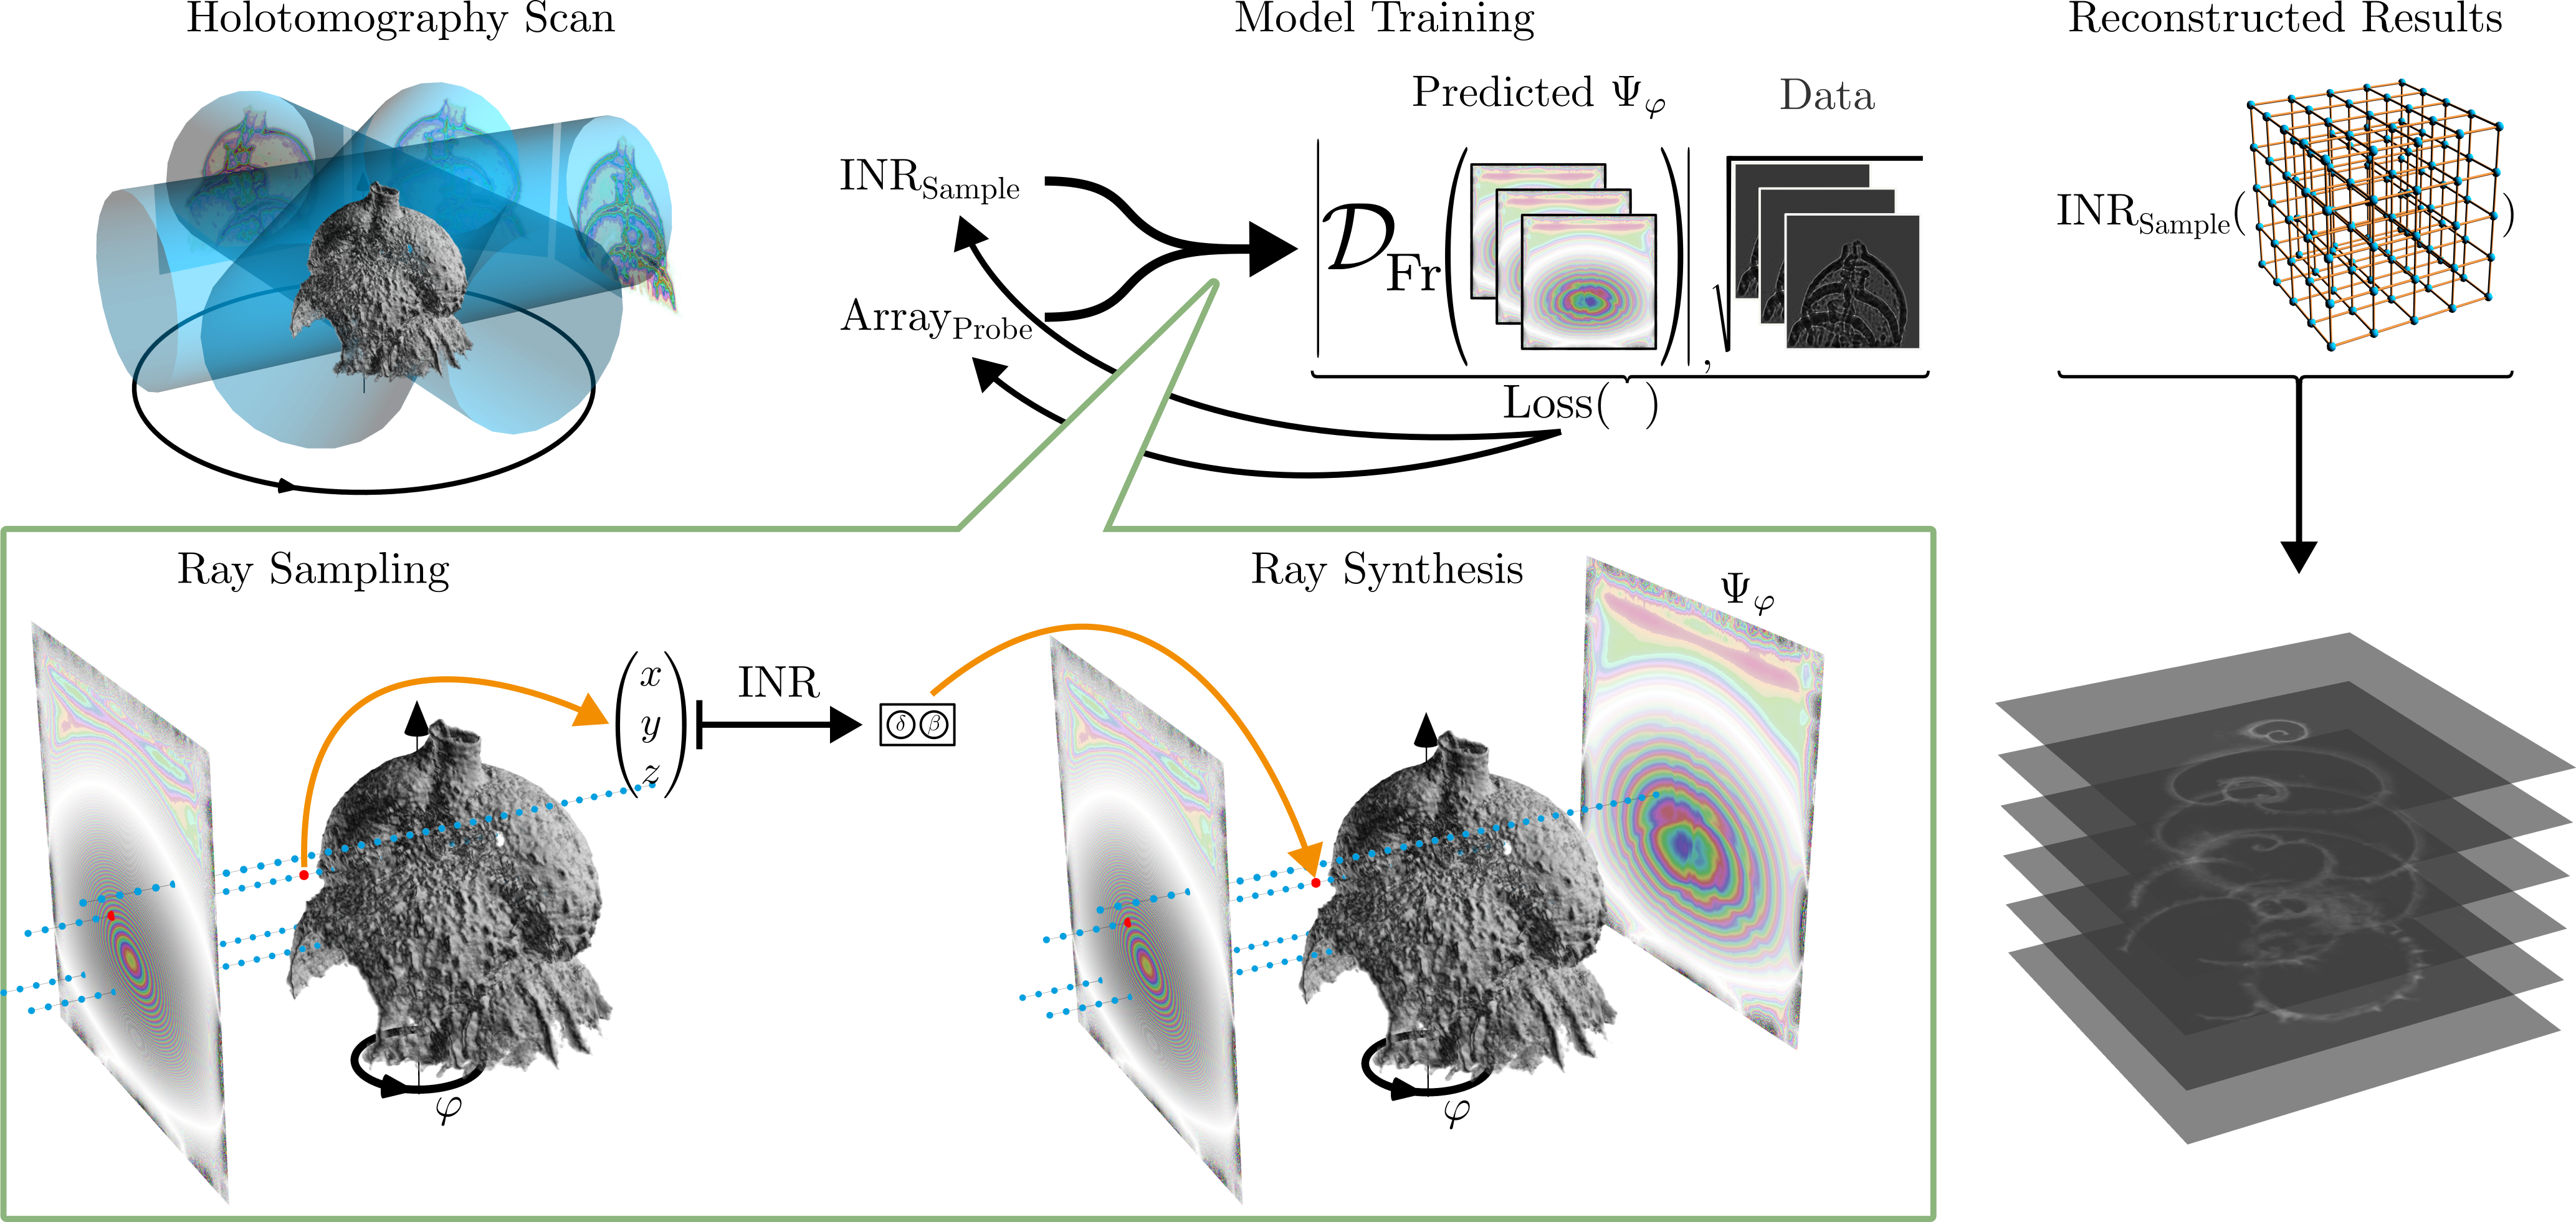
\includegraphics[width=\textwidth]{imgs/physics+INR.png}
 \caption[Illustration of the used architecture.]{
  The training scheme.
  Given a holotomography data set, we use the INR and the array modeling the probe to obtain the exiting wave field which we propagate and compare to the data.
  After training the INR can be queried at a grid to get a 3D volume.
}
 \label{fig:training_scheme}
\end{figure}\\
We update all the parameters after the loss is evaluated for one angle.
For the hyperparameter in the loss function \eqref{eq:loss_fct} we can say that \(  \alpha_{1} \) has to be chosen large enough that probe and sample are separated and should be weighted more than the data fidelity.
For the other two, there is a trade-off between the bias introduced by these regularizers and their positive effect on the reconstructions, therefore the choice is not trivial and depends on the quality of the measurements and the structure of object and probe.
Regularization strategies we apply in the following include \( L_{1}, L_{2} \) and \(  TV \) regularization, as well as the term
\begin{equation}
R_{\delta,\beta} (O) = \left\| \left| \frac{\delta}{\beta} \right| - \max \left(  b, \left| \frac{\delta}{\beta} \right| \right)  \right\|_{L_2}^2 +  \left\| \left| \frac{\beta}{\delta} \right| - \max \left(   \frac{1}{a}, \left| \frac{\beta}{\delta} \right| \right) \right\|_{L_2}^2, 
  \label{eq:d/b_regularization}
\end{equation}
which supports an explicit connection the phase shift and absorption of our object \(  O  \).
The values \( a, b \in \mathbb{R} \) are chosen such that we expect \( \frac{\delta}{\beta} \in \left[ a,b \right]  \) depending on the materials we might know and the X-ray energy, but allows for different materials in comparison to other reconstruction methods \cite{villanueva-perezContrasttransferfunctionPhaseRetrieval2017}.
\\
One challenge in our optimization process is that the pixels in the rendered projections interact with each other when the waves are propagated through free space, i.e.
we cannot evaluate the rays independently in measurement space as it is possible for computed tomography \cite{zhaNAFNeuralAttenuation2022}.\\
Hence, we need to sample \( n \cdot  n \) rays (\(  n^3 \) points) for \( \mathcal{I}_\mathrm{det} \in \mathbb{R}^{n \times n} \) which are then projected and propagated to compare them to the measurements.
As this becomes extremely memory demanding for highly resolved data, we limit the number of rays for which we calculate gradients to update the INR to \( C_\mathrm{VRAM} \approx 8000 \).
The progress for large \(  n \) is still slow due to two reasons.
Firstly we scale the number of points on the ray according to the resolution, i.e. \( \left| \ell_{x,y,\varphi} \right| = n  \), and secondly only \( C_\mathrm{VRAM} \) of the \(  n^2 \) rays (below 1\% for \( n>1000 \)) are used to update the INR.
But we can accelerate everything massively by using a multi-scale approach similar to \cite{doraArtifactsuppressingReconstructionStrongly2024}, which gives reasonable results after short time that serve as initialization for higher resolutions.
Especially the reconstruction of bigger structures and separation between object and background work well on lower resolutions.\\
To make the training more stable, we use gradient clipping with which we limit the gradient norm to five times the median of the 100 previous gradient norms. Additionally we use a learning rate scheduler that halves the step size when the loss does not decrease anymore and ultimately stops if the learning rate reaches \( 10^{-7} \).
\\
Our implementation relies on \textit{PyTorch} and \textit{tiny-cuda-nn} \cite{paszkePyTorchImperativeStyle2019, tiny-cuda-nn}.

